\begin{flushright} {\tiny {\color{gray} basis\_Pm1\_2D.tex}} \end{flushright}
%~~~~~~~~~~~~~~~~~~~~~~~~~~~~~~~~~~~~~~~~~~~~~~~~~~~~~~~~~~~~~~~~~~~~~~~~~~~~~~~~~~~~~~~~~~~~~~~~~~

On the reference element $\Omega=[-1,1]\times[-1,1]$ we have three nodes placed as follows:

\begin{flushright} {\tiny {\color{gray} (tikz\_pm1\_2D.tex)}} \end{flushright}
%~~~~~~~~~~~~~~~~~~~~~~~~~~~~~~~~~~~~~~~~~~~~~~~~~~~~~~~~~~~~~~~~~~~~~~~~~~~~~~~~~~~~~~~~~~~~~~~~~~

\begin{center}
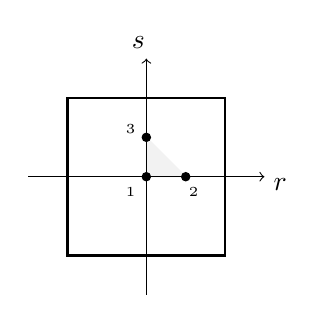
\begin{tikzpicture}
%\draw[step=0.5cm,gray,very thin] (0,0) grid (4,4); 
\draw[fill=gray!10,gray!10](2,2)--(2.5,2)--(2,2.5)--cycle;
\draw[thick] (1,1)--(3,1)--(3,3)--(1,3)--cycle;
\draw [->] (0.5,2) -- (3.5,2);
\draw [->] (2,0.5) -- (2,3.5);
\node[] at (3.7,1.9) {$r$};
\node[] at (1.9,3.7) {$s$};
\draw[black,fill=black] (2,2)   circle (1.5pt);
\draw[black,fill=black] (2.5,2)   circle (1.5pt);
\draw[black,fill=black] (2,2.5)   circle (1.5pt);
\node[] at (1.8,1.8) {\tiny $1$};
\node[] at (2.6,1.8) {\tiny $2$};
\node[] at (1.8,2.6) {\tiny $3$};
\end{tikzpicture}
\end{center}



Let us assume that the function $f(r,s)$ is to be approximated on $[-1,1]\times[-1,1]$ by 
\[
f^h(r,s)=a+br+cs
\]
Note that this is a linear function, not a bilinear one. 
The function $f^h$ then must fulfill:
\begin{eqnarray}
f^h(r_1,s_1)&=&a \;\;\;\;\;\; =f_1    \nn\\
f^h(r_2,s_2)&=&a+\frac{b}{2}=f_2 \nn\\
f^h(r_3,s_3)&=&a+\frac{c}{2}=f_3 \nn
\end{eqnarray}
This leads to : 
\[
a=f_1
\quad
\quad
b=2(f_2-f_1)
\quad
\quad
c=2(f_3-f_1)
\]
Then
\[
f(r,s)=f_1 + 2(f_2-f_1) r + 2(f_3-f_1) s
\]
or, 
\[
f(r) = \sum_{i=1}^3 N_i(r,s) f_i
\]
with
\begin{mdframed}[backgroundcolor=blue!5]
\begin{eqnarray}
\bN_1(r) &=& 1-2(r+s)  \nonumber\\
\bN_2(r) &=& 2r   \nonumber\\
\bN_3(r) &=& 2s
\end{eqnarray}
\end{mdframed}

Note that we could also have placed the nodes at a different location: 

\begin{flushright} {\tiny {\color{gray} (tikz\_pm1\_2D\_bis.tex)}} \end{flushright}
%~~~~~~~~~~~~~~~~~~~~~~~~~~~~~~~~~~~~~~~~~~~~~~~~~~~~~~~~~~~~~~~~~~~~~~~~~~~~~~~~~~~~~~~~~~~~~~~~~~

\begin{center}
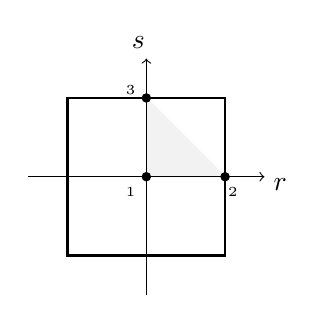
\begin{tikzpicture}
%\draw[step=0.5cm,gray,very thin] (0,0) grid (4,4); 
\draw[fill=gray!10,gray!10](2,2)--(3,2)--(2,3)--cycle;
\draw[thick] (1,1)--(3,1)--(3,3)--(1,3)--cycle;
\draw [->] (0.5,2) -- (3.5,2);
\draw [->] (2,0.5) -- (2,3.5);
\node[] at (3.7,1.9) {$r$};
\node[] at (1.9,3.7) {$s$};
\draw[black,fill=black] (2,2)   circle (1.5pt);
\draw[black,fill=black] (3,2)   circle (1.5pt);
\draw[black,fill=black] (2,3)   circle (1.5pt);
\node[] at (1.8,1.8) {\tiny $1$};
\node[] at (3.1,1.8) {\tiny $2$};
\node[] at (1.8,3.1) {\tiny $3$};
\end{tikzpicture}
\end{center}



and we would then have
\begin{mdframed}[backgroundcolor=blue!5]
\begin{eqnarray}
\bN_1(r) &=& 1-r-s  \nonumber\\
\bN_2(r) &=& r   \nonumber\\
\bN_3(r) &=& s
\end{eqnarray}
\end{mdframed}






